\documentclass[12pt]{article}
\usepackage{lingmacros}
\usepackage{tree-dvips}
\usepackage[utf8x]{inputenc} % Включаем поддержку UTF8 
\usepackage[russian]{babel} 
\usepackage{mathtools}
\usepackage{graphicx}
\usepackage{amsmath}

\graphicspath{{pict/}}
\DeclareGraphicsExtensions{.pdf,.png,.jpg}

\DeclarePairedDelimiter{\ceil}{\lceil}{\rceil}

\begin{document}

\section*{Решения}

\subsection*{Задача 2.1}
За один вопрос можно сократить перебираемое множество вдвое. Таким образом, достаточно двух вопросов. Ответ: 2.

\subsection*{Задача 2.2}
Подставим точки в уравнение и решим систему:

\begin{equation*} 
    \begin{cases}
    1 = a\cdot 0^2 + b\cdot 0 + c,\\
    2 = a\cdot 1^2 + b\cdot 1 + c,\\
    1 = a\cdot 2^2 + b\cdot 2 + c;
    \end{cases}
\end{equation*}

\begin{equation*} 
    \begin{cases}
    c = 1,\\
    a + b = 1,\\
    2a + b = 0;
    \end{cases}
\end{equation*}

\begin{equation*} 
    \begin{cases}
        a = -1,\\
        b = 2, \\
        c = 1. \\
    \end{cases}
\end{equation*}

Уравнение параболы с вычисленными коэффициентами $y = -x^2 + 2x + 1$. Найдем абсциссу точки перегиба: 
$$y'_x=0 \Leftrightarrow -2x + 2 = 0 \Leftrightarrow x = 1. $$
При x = 1 y = 2. Ответ: (1, 2).

\subsection*{Задача 2.3}
Выразим корень уравнения: $x = -A/3$. Таким образом, $x \in [-2/3, -1/3]$. Значит $$P(x \in [-2/3, -0.4]) = \frac{-0.4+2/3}{1/3} = 2 - 1.2 = 0.8.$$ Ответ: 0.8.

\subsection*{Задача 2.4}
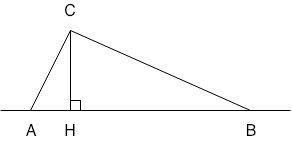
\includegraphics{math24}\\
Наикратчайший путь равен длине перпендикуляра, опущенного из вершины $C$ к прямой $AB$. По длинам сторон очевидно, что $\triangle ABC$ -- прямойгольный, с прямым углом в вершине $C\space (7^2 + 24^2 = 25^2)$. Так, согласно свойству прямоугольного треугольника, $CH = AC\cdot BC / AB = 6.72$. Ответ: 6.72.
\subsection*{Задача 2.5}
В данной задаче необходимо найти такое натуральное максимальное $n$, при котором $\exists a \forall x \in N: x < n \Rightarrow x < a^x < x + 1$. Выпишем границы интервалов $(\sqrt[x]{x}, \sqrt[x]{x + 1})$ для нескольких первых значений $x$.\\
\begin{tabular}{l l l}
    x & \text{Левая граница a} & \text{Правая граница a} \\
    $1$ & $1$ & $2$ \\
    $2$ & $\sqrt[2]{2} = 1.41421356$ & $\sqrt[2]{3} = 1.73205081$\\
    $3$ & $\sqrt[3]{3} = 1.44224957$ & $\sqrt[3]{4} = 1.58740105$\\
    $4$ & $\sqrt[4]{4} = 1.41421356$ & $\sqrt[4]{5} =  1.49534878$\\
    $5$ & $\sqrt[5]{5} = 1.37972966$ & $\sqrt[5]{6} = 1.43096908$\\
    \dots & \dots & \dots \\
\end{tabular}\\
По таблице видно, что $\sqrt[5]{6} < \sqrt[3]{3}$. Таким образом, $n = 4$ -- наибольшее значение, удовлетворяющее условию задачи. Ответ: 4.

\subsection*{Задача 2.6}
В данной задаче надо проверить делимость произведения чисел. $x\cdot (x + 2)\cdot(x + 3) \cdot (x + 4)$ гарантированно делится на $2$ и на $3$, так как содержит произведение последовательно идущих $3$ чисел. Делимость на остальные числа при любом $x$ гарантировать нельзя. Ответ: 6.

\subsection*{Задача 2.7}
Первый может выбросить $9$ различных наборов (последовательность не учитывается). Если в наборе $x$ орлов, то количество возможных вариантов второго игрока, удовлетворяющих условию $(9 - x)$. Всего возможных способов выкинуть наборы у обоих игроков: $9 \cdot 10 = 90$. $$P = \frac{\sum\limits_{x=0}^8{9-x}}{90}=0.5.$$
Ответ: 0.5.  
\subsection*{Задача 2.8}
Постепенно раскрывая скобки найдем сумму коэффициентов полинома $(x^2-3x+1)^n$ для $n$, начиная с 1.\\
\begin{tabular}{l l}
    $n$ & Сумма коэффициентов \\
    $1$ & $-1$  \\
    $2$ & $1$  \\
    $3$ & $-1$  \\
    $4$ & $1$  \\
    \dots & \dots \\
\end{tabular}\\
Подметим, что при нечётном $n$ сумма коэффициентов равна $-1$, а при чётном -- $1$. Ответ: 1.

\subsection*{Задача 2.9}
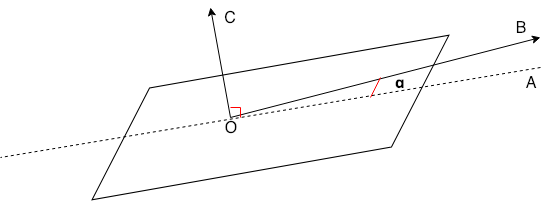
\includegraphics{math29}\\
$$\cos\alpha = \frac{|(\vec{OB}, \vec{OC})|}{|\vec{OB}|\cdot|\vec{OC}|} = \frac{20}{\sqrt{25+144}\sqrt{16+9}}= \frac{4}{13},$$
$$\sin\alpha = \sqrt{1 - \cos^2 \alpha = 0.9514859}.$$\\
Ответ: 0.9514859.
\subsection*{Задача 2.10}
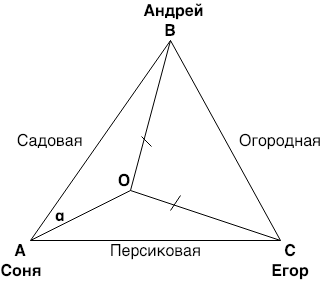
\includegraphics{math210}\\
Обозначим искомый угол буквой $\alpha$. $\angle BAC = 45^\circ \Rightarrow \angle OAC = 45^\circ - \alpha$. $\angle OCA = 15^\circ \Rightarrow \angle AOC = 120^\circ + \alpha$. $\angle OCB = \angle OBC = 60^\circ - 15^\circ = 45^\circ \Rightarrow \angle BOC = 90^\circ$. $\angle ABO = 30^\circ$. По теореме синусов:
$$\frac{\sin\alpha}{OB} = \frac{\sin 30^\circ}{AO} \Rightarrow AO = \frac{OB}{2\sin\alpha}$$
$$\frac{\sin 15^\circ}{OA} = \frac{\sin (45^\circ - \alpha)}{OC} \Rightarrow AO = \frac{OC\sin 15^\circ}{\sin (45^\circ - \alpha)}$$ \\
Так как $OB = OC$, 
$$\sin (45^\circ - \alpha) = 2\sin\alpha \sin 15^\circ \Rightarrow \alpha = 30^\circ.$$\\
Ответ: 30.
\end{document}